% ==================================================
% CHAPTER 3: The New Small Wheels %
% ==================================================

\chapter{The New Small Wheels}
\label{chap:nsw}
% Edit count: Lia - 0, Brigitte - 0

% --------------------------------------------------
\section{Motivation for the New Small Wheels (NSWs)}
% --------------------------------------------------

The hit rate of all detector systems will increase with the HL-LHC not only because of the increase in luminosity, but also because the background radiation rate increases linearly with luminosity.
The combined rate presents problems for both the tracking and triggering capabilities of the muon spectrometer~\cite{nsw_tdr}.

In term of tracking, the efficiency of the MDTs decreases by 35\% (mostly due to long dead-times) already when exposed to the maximum hit rate at the current luminosity, 300 kHz.
At the threefold increase in luminosity predicted for run-3, most of the small wheel will be subjected to a hit rate well above 300 kHz and it will begin missing hits. Losing hits in the small wheel will reduce the high $p_T$ muon momentum resolution. The decrease in resolution will affect the ability to search for, for example, high mass $Z'$, $W'$ and pseudo-scalar Higgs~\cite{nsw_tdr}.

Already, the forward muon trigger system copes with a very high fake rate, even when including TGC data from the small wheel in the trigger as in run-2. At the luminosity expected in run 3, 60 kHz of the maximum 100 kHz of the L1 trigger would be taken by the endcap muon spectrometer. A possible solution would be to raise the minimum $p_T$ threshold from \SI{20}{\giga\electronvolt} to \SI{40}{\giga\electronvolt}, but the ability to study several physics processes of interest depend on low $p_T$ muons, particularly Higgs decays and SUSY particle decays to leptons~\cite{nsw_tdr}.

The NSW will solve both these problems. It will be covered with precision tracking chambers suitable for the expected hit rates and triggering chambers capable of \SI{1}{mrad} angular resolution. The idea behind the triggering chambers is to match the small wheel track segment with the track segment from the big wheel to discard tracks not originating from the interaction point. Figure~\ref{fig:nsw_track_triggering} illustrates this point: the run-1 trigger system would have triggered on all three tracks, while with the NSW the trigger system would only trigger on track A~\cite{nsw_tdr}.

% Currently, the small wheel is made of thin-gap chambers, which record hits. They have the known problem that particles generated in the material of the end-cap toroid magnet that hit the small wheel cannot be distinguished from muons from the interaction point. For example, in figure~\ref{fig:nsw_track_triggering}, all three tracks would be triggered on.

\begin{figure}
    \centering
    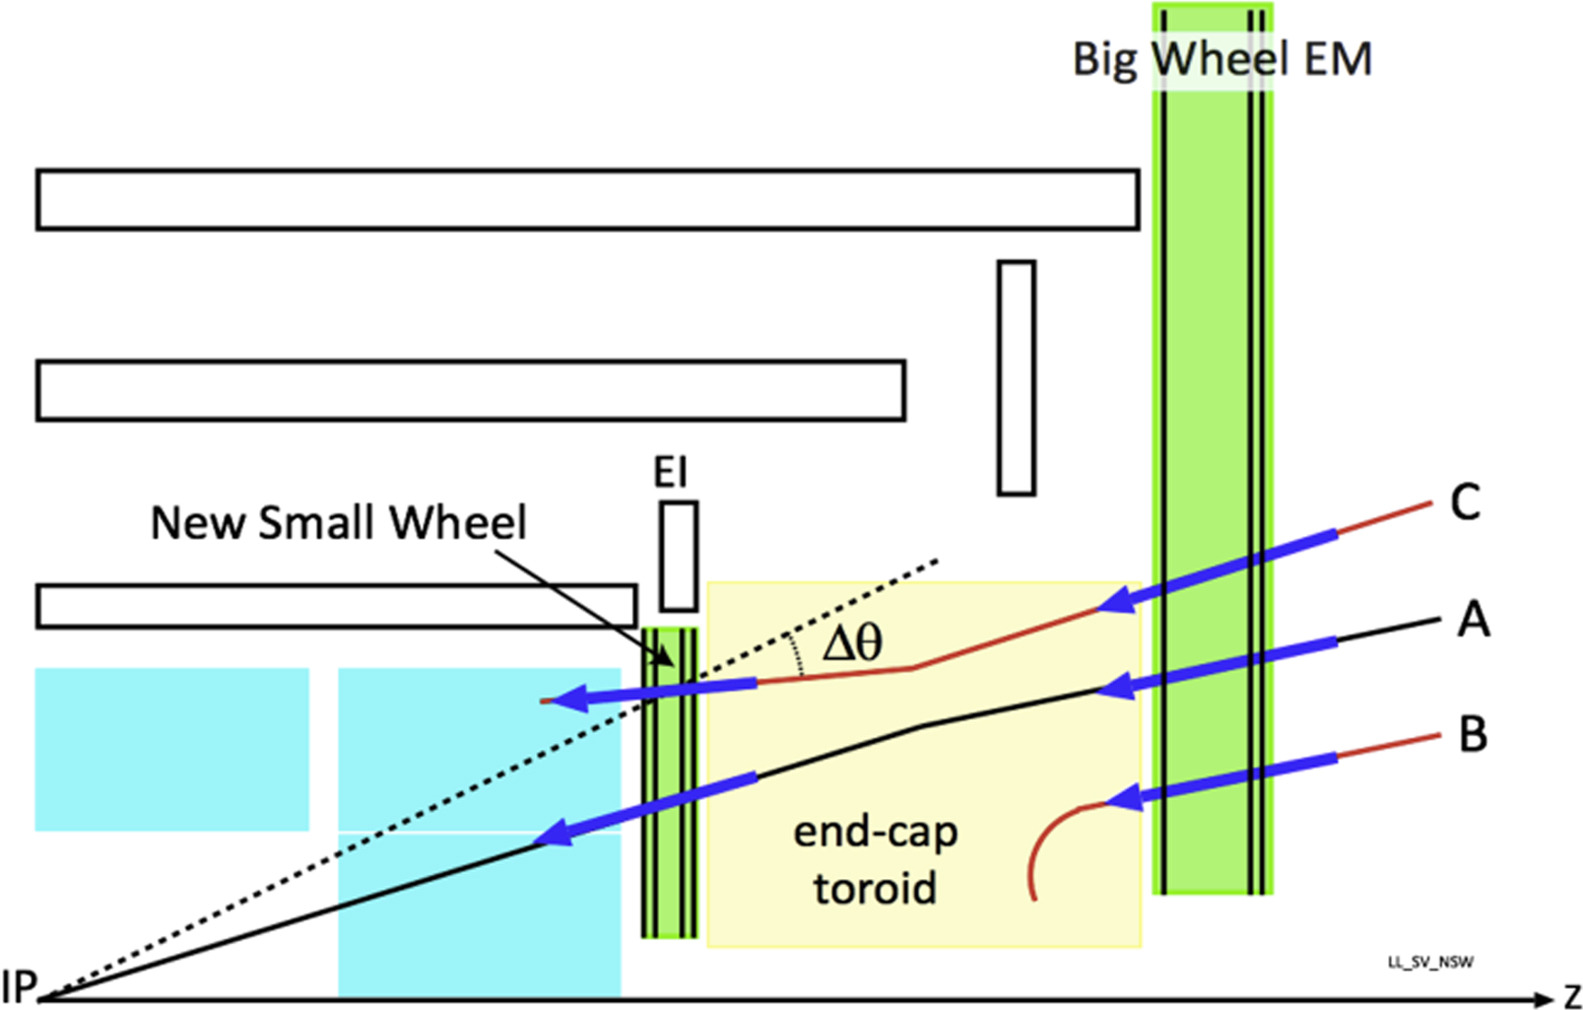
\includegraphics[width = 0.9\textwidth]{figures/perez-codina_NSW_tracks.jpg}
    \caption{A schematic of a quarter cross section of the ATLAS detector, with the collision/interaction point (IP) in the bottom left corner. Three possible tracks are labelled. Ideally, track A would be triggered upon while track B and C discarded. With the small wheel, all three tracks would be recorded. With the NSW, only track A would be recorded~\cite{nsw_tdr}.}
    \label{fig:nsw_track_triggering}
\end{figure}

% --------------------------------------------------
\section{Design of the NSWs}
% --------------------------------------------------

The NSWs are covered with two detector technologies: micromegas (MM) and small-strip thin gap chambers (sTGCs). MMs are the primary tracking detectors and sTGCs are the primary triggering detectors, but for redundancy sake both are designed to do either. As such, both sets of detectors are to have position resolution better than $\sim$\SI{100}{\micro\meter} per plane. Four chambers of each type are glued together to create quadruplet modules. Quadruplets of different sizes are assembled into wedges. Two sTGC wedges and two MM wedges are layered to create sectors (with the sTGC wedges on the outside)~\cite{nsw_tdr}. Different stages of the constrcution process are shown in figure~\ref{fig:nsw_breakdown}.% \textcolor{red}{\textit{for if you use computer generated NSW diagram}} Sectors covered the wheel, as shown in figure~\ref{fig:nsw_diagram}. Practically, two different wedge sizes, small and large, were required to completely cover the wheel.
% \begin{figure}
%    \centering
%    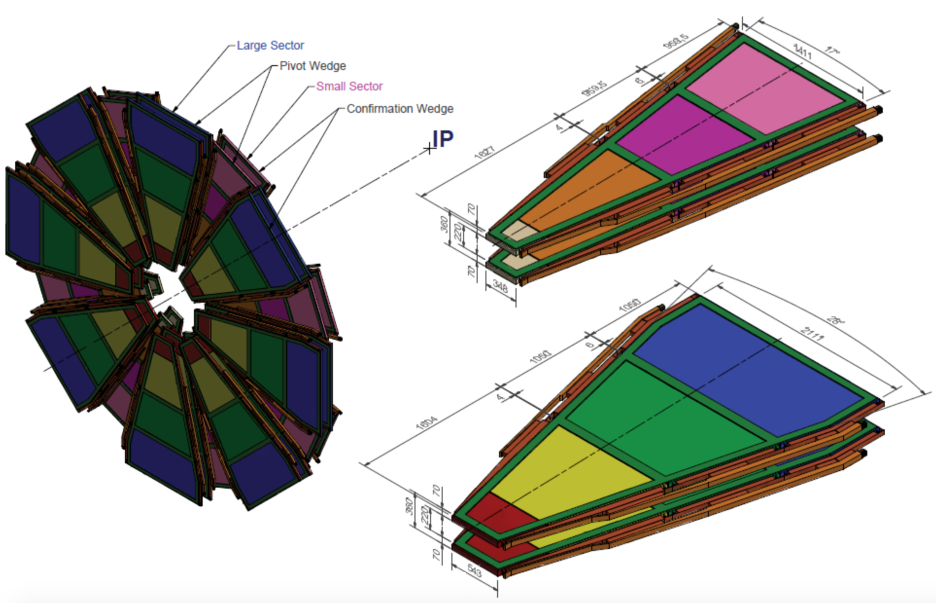
\includegraphics[width = 0.9\textwidth]{figures/nsw_diagram.png}
%    \caption{Drawing of the new small wheel, and diagrams of the individual small and large wedges. Each colour represents a different sTGC module size.}
%    \label{fig:nsw_diagram}
% \end{figure}
\newpage
\thispagestyle{empty}
\newgeometry{top=0.5in,bottom=0.5in}
\begin{figure}
\centering
\begin{subfigure}{\textwidth}
  \centering
  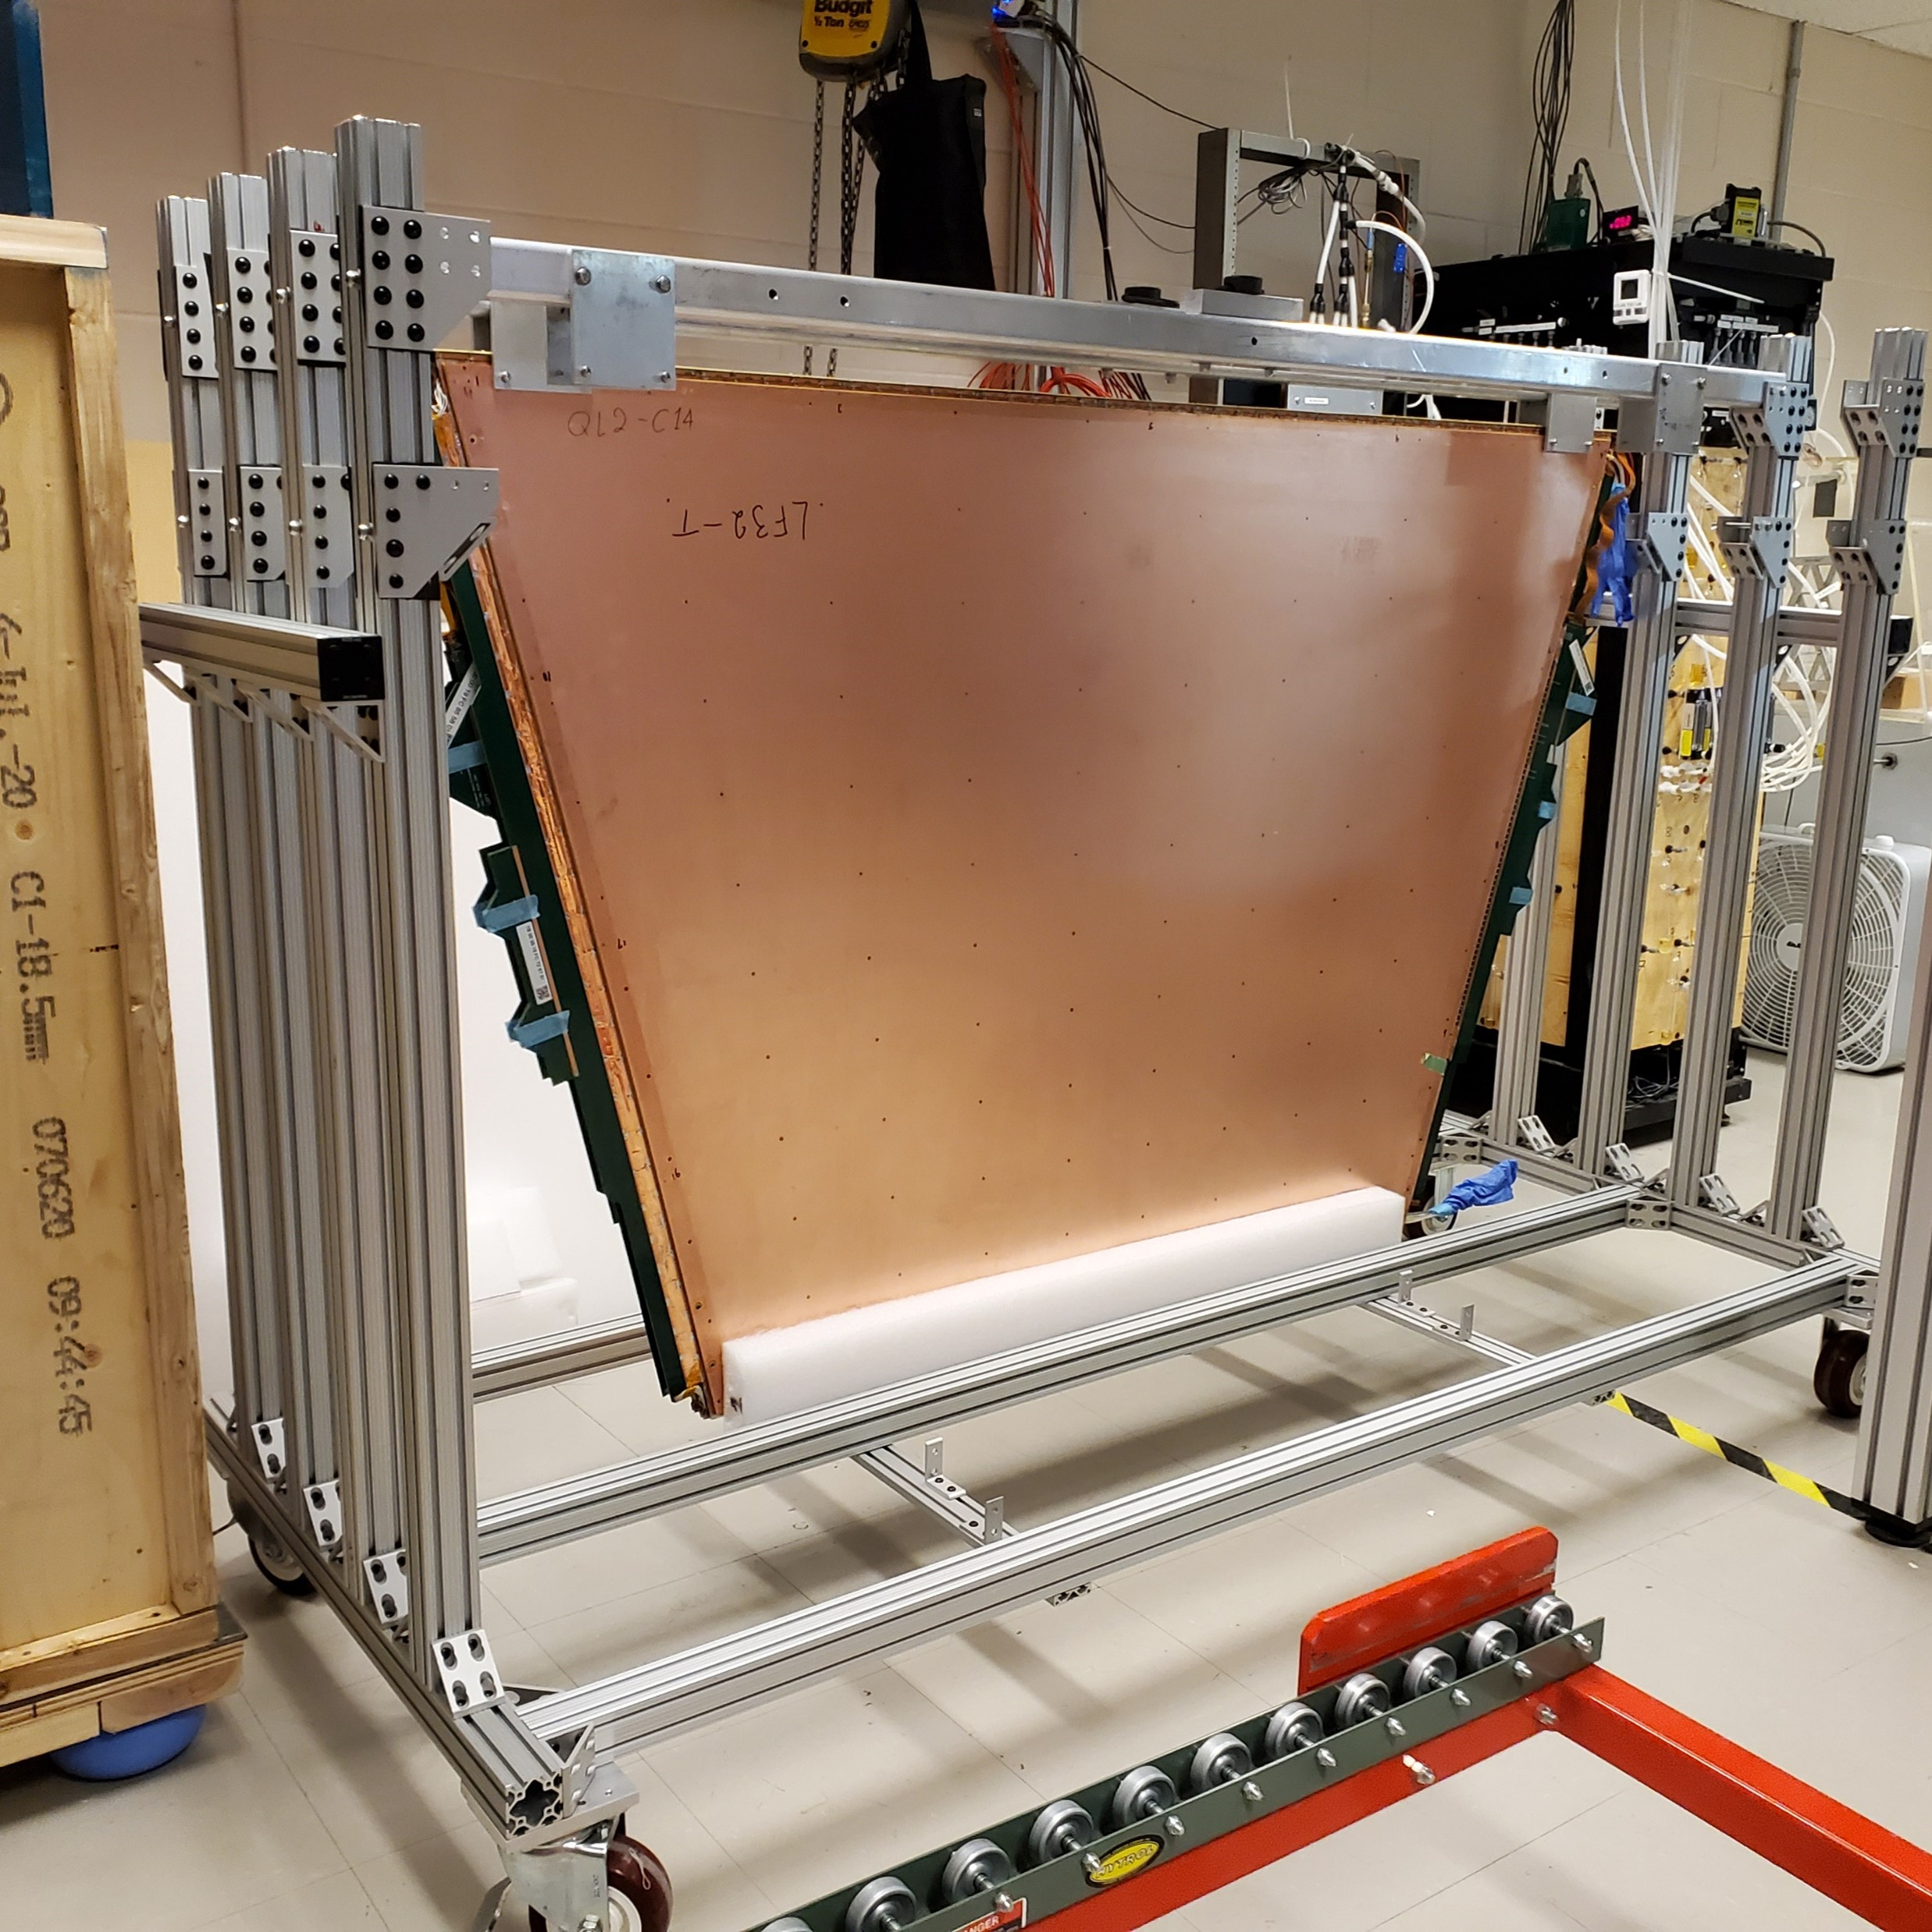
\includegraphics[width=0.35\textwidth]{figures/stgc_quad_cart.jpg}
  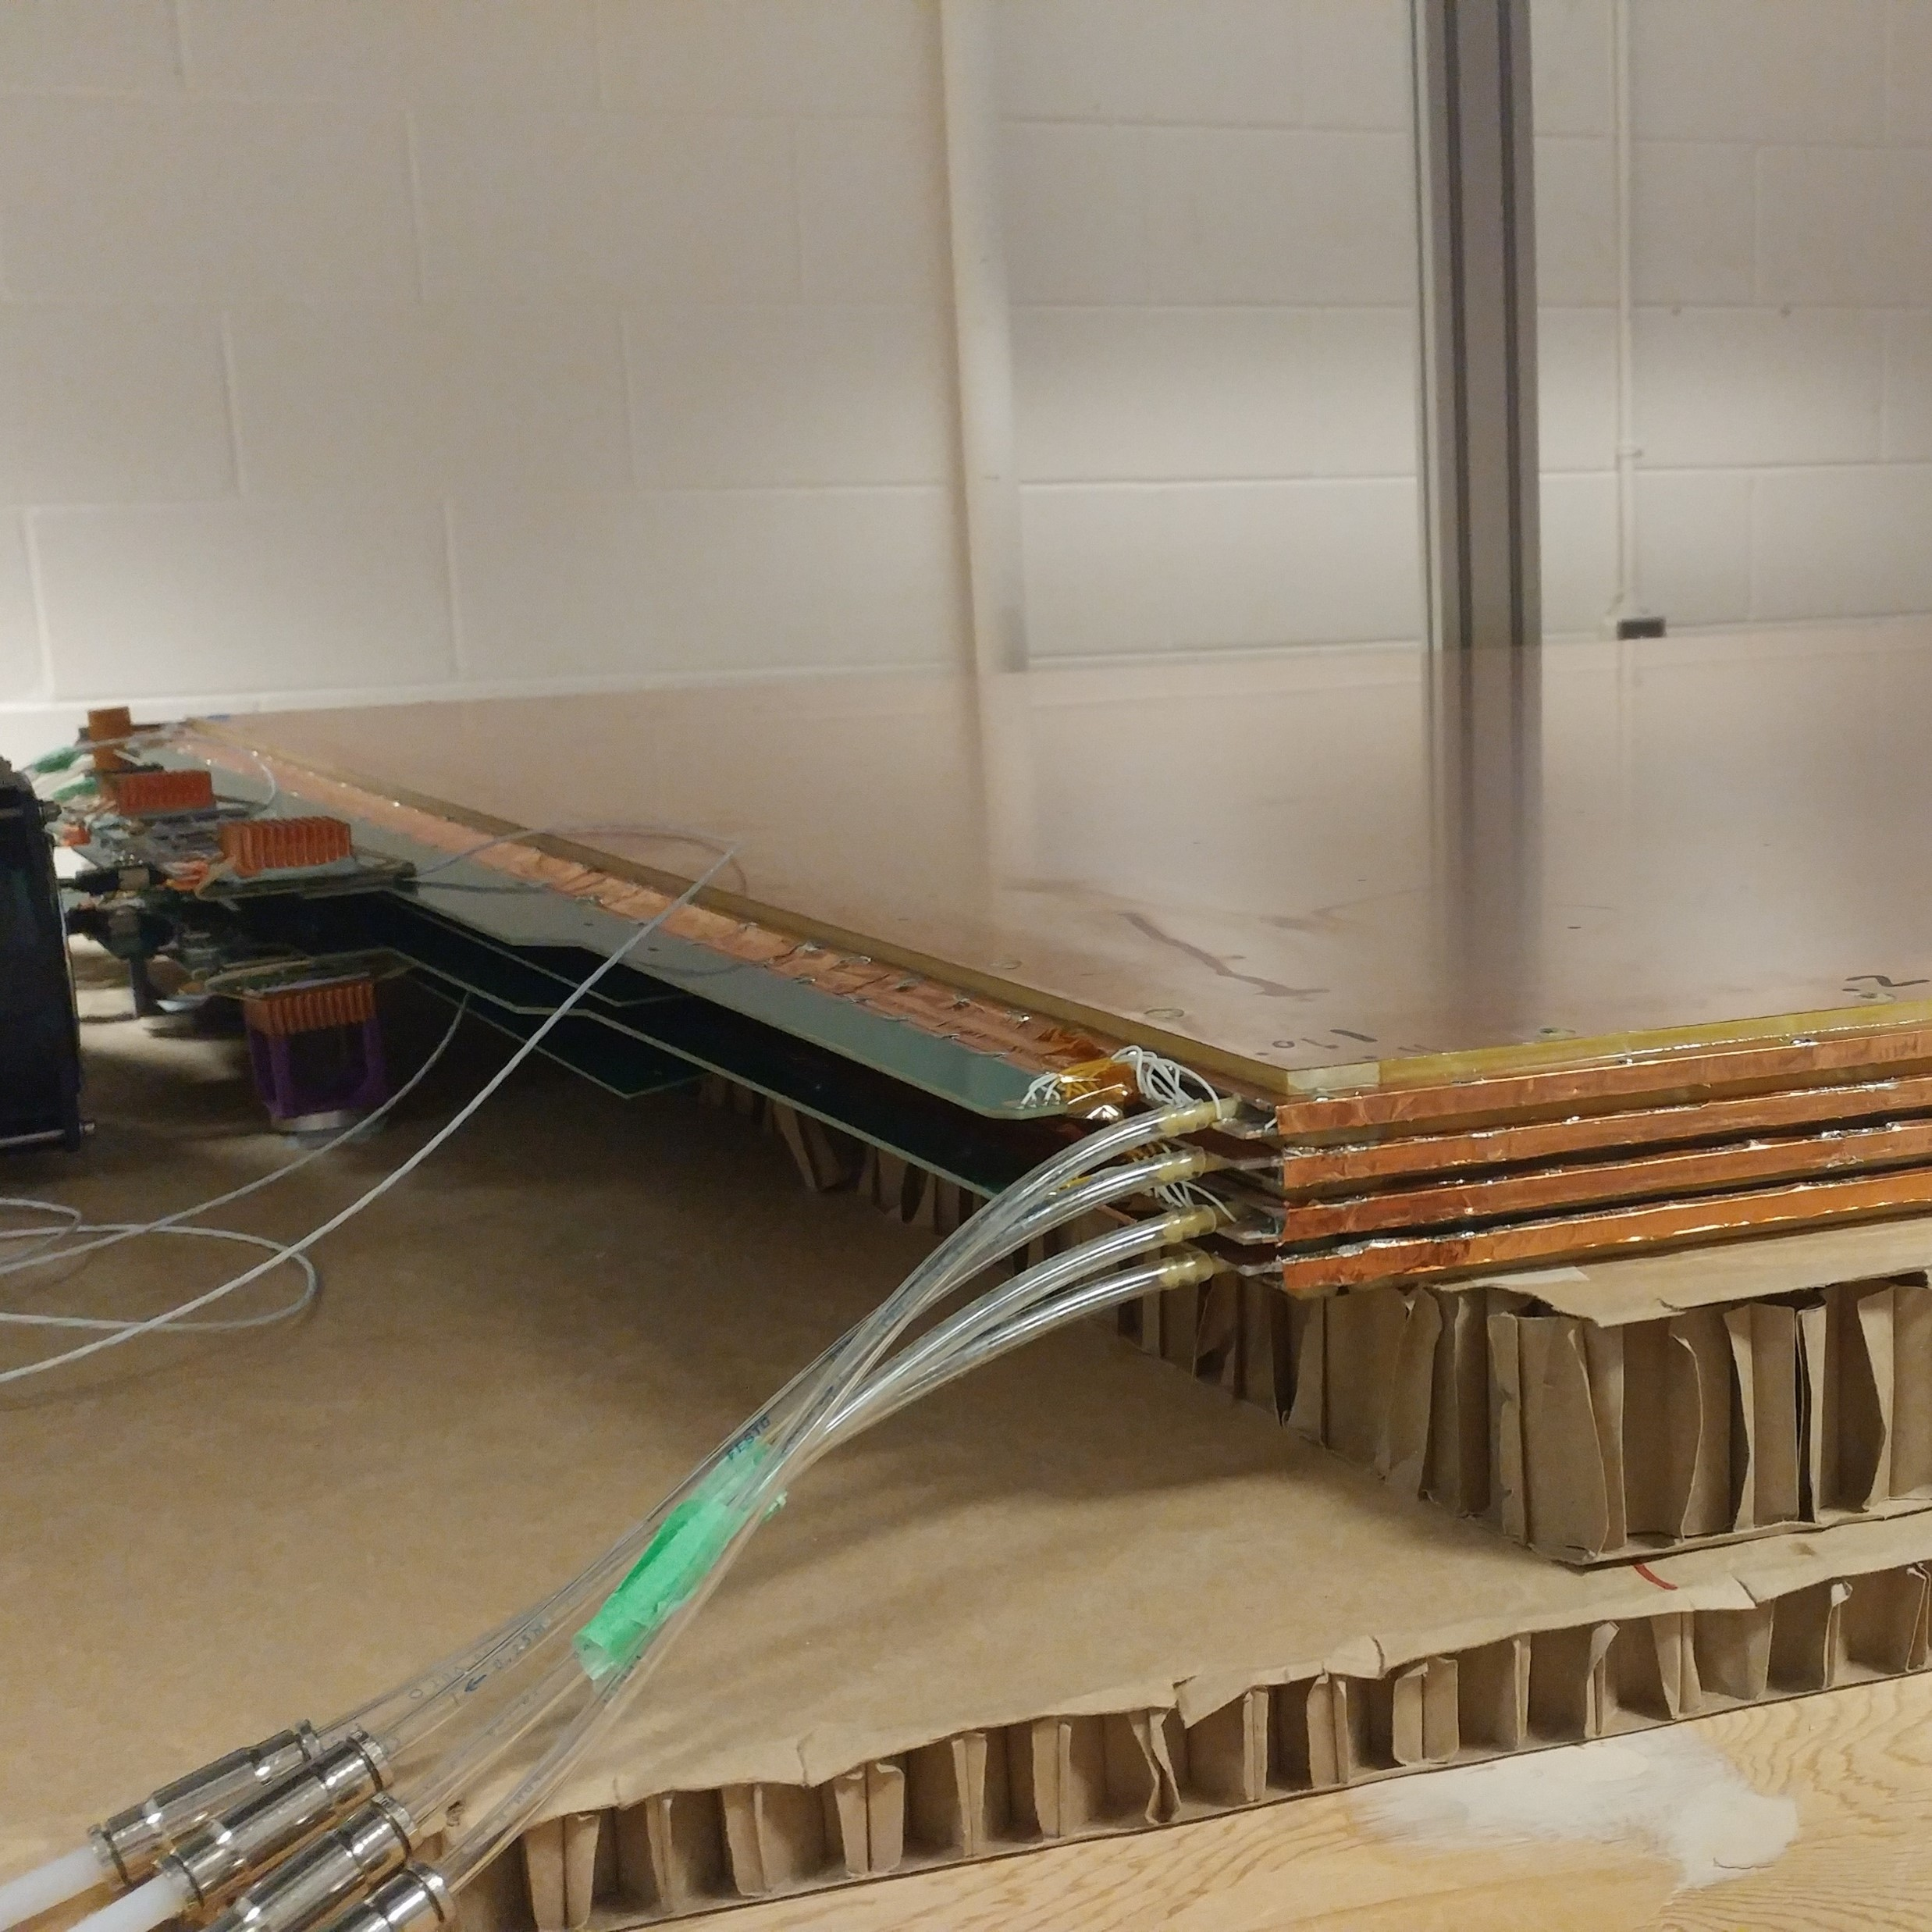
\includegraphics[width=0.35\textwidth]{figures/stgc_quad_inlet_corner.jpg}
  \caption{An sTGC quadruplet module. The left image highlights the trapezoidal shape. The right image shows the short edge corner. The four sTGC layers and each layer's gas inlet are visible. The gas outlets and high voltage cables are at the long edge in the back of the photo. The green printed circuit board along the sides are the adaptor boards where the front end electronics are attached.}
  \label{fig:stgc_quad}
\end{subfigure}

\smallskip

\begin{subfigure}{\textwidth}
  \centering
  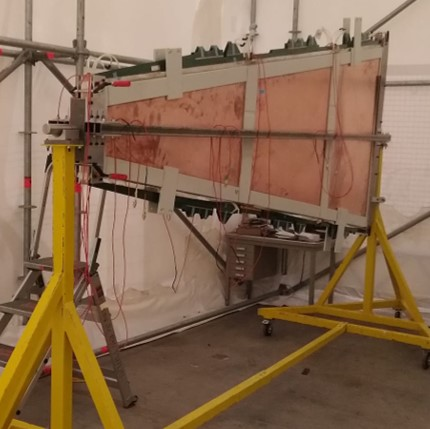
\includegraphics[width=0.35\textwidth]{figures/stgc_wedge.jpg}
  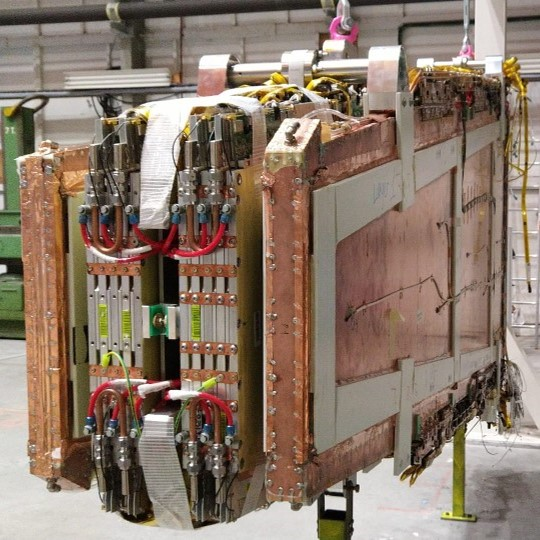
\includegraphics[width=0.35\textwidth]{figures/sector.jpg}
  \caption{Left: An sTGC wedge. The white frame outlines the individual quadruplet modules. Right: A completed sector, with two sTGC wedges on the outside and two MM wedges on the inside.}
  \label{fig:wedge_and_sector}
\end{subfigure}

\smallskip

\begin{subfigure}{\textwidth}
  \centering
  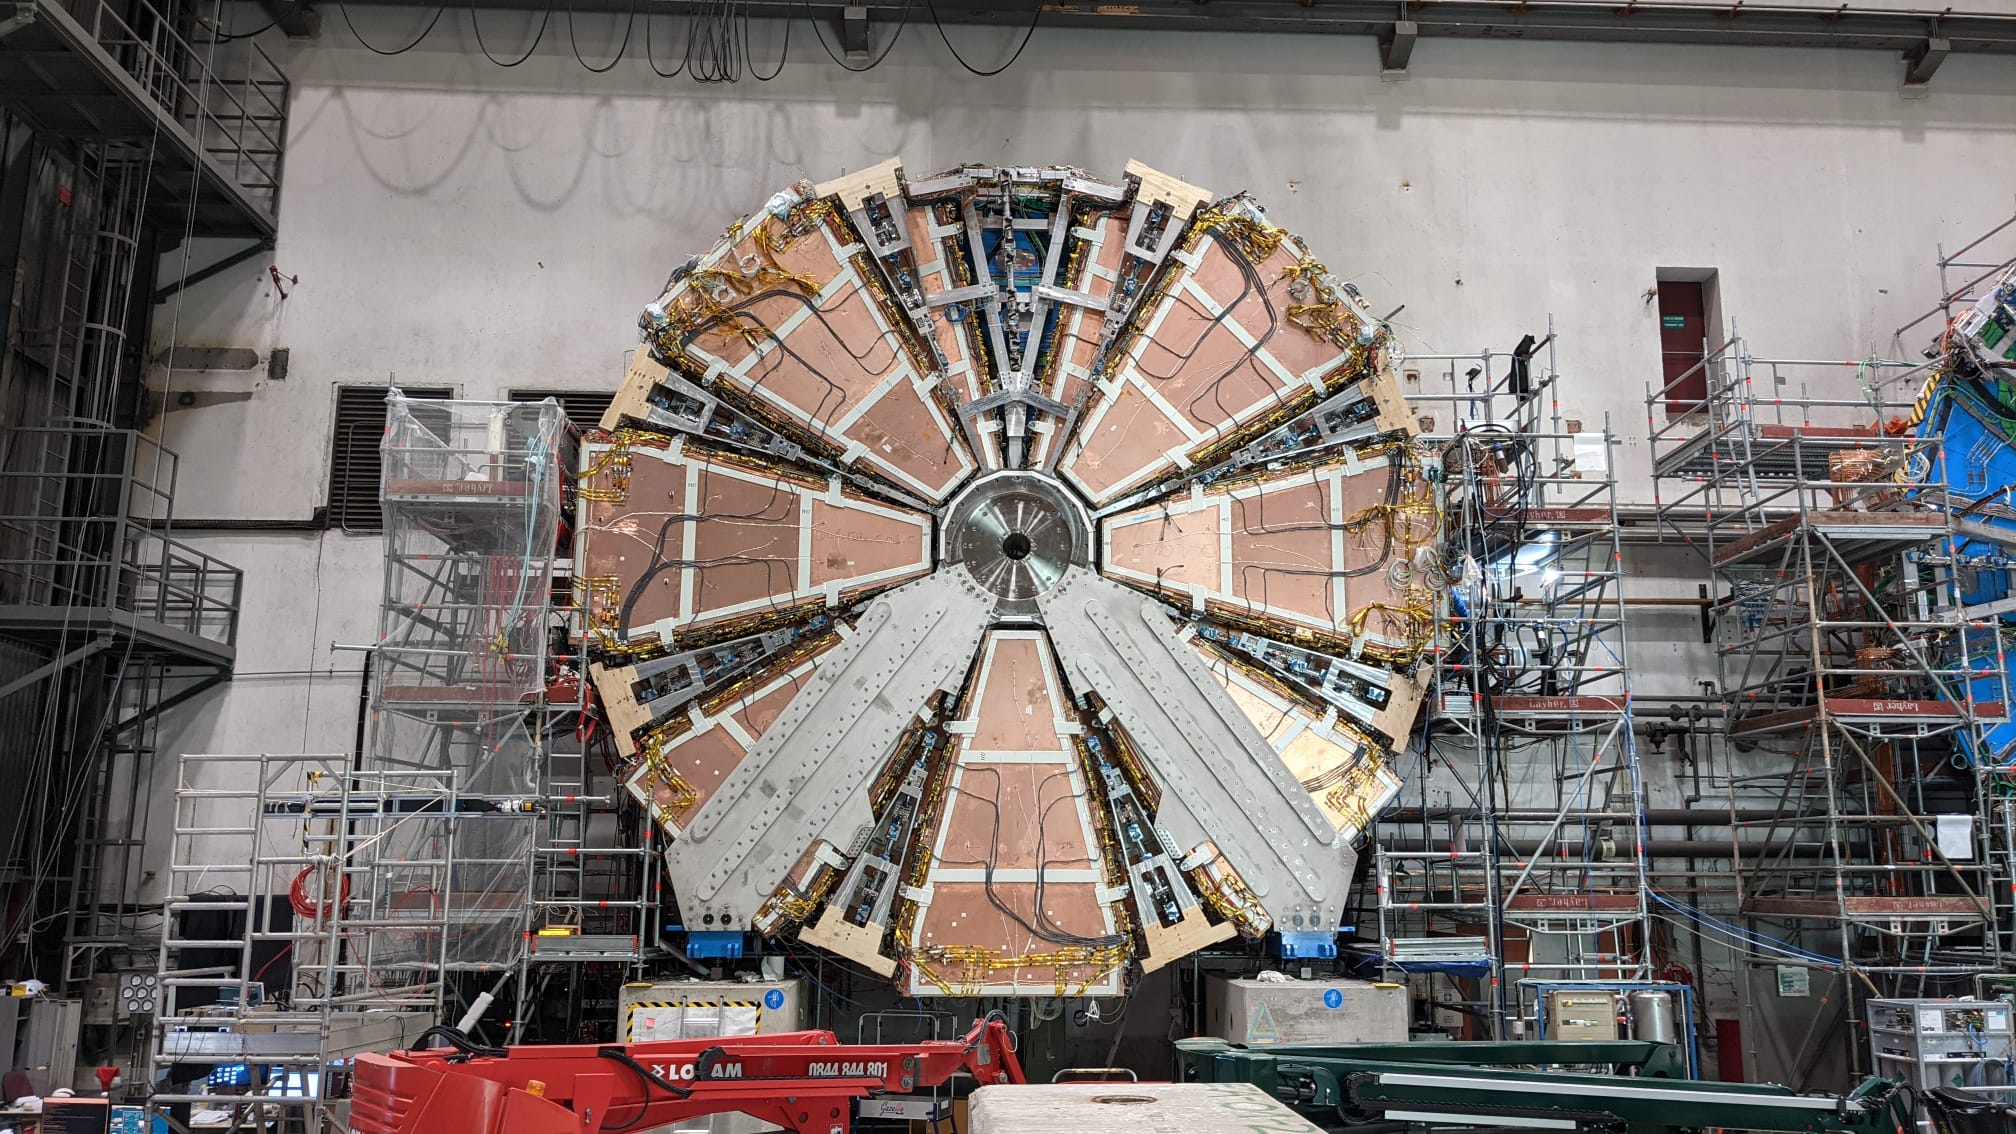
\includegraphics[width=0.7\textwidth]{figures/nsw_2021-05-27_landscape.jpeg}
  \caption{The new small wheel. All sectors except one large sector at the top are installed, revealing two of the smaller sectors that are normally hidden under the large sectors and support bars. The NSWs are \SI{10}{m} in diameter. }
  \label{fig:nsw}
  \end{subfigure}
\caption{Images breaking down some of the construction units of the NSWs.}
\label{fig:nsw_breakdown}
\end{figure}
\newpage
\restoregeometry

%TODO : Pivot vs confirm? You don't mention the difference anywhere.

% --------------------------------------------------
% \section{Micromegas}
% --------------------------------------------------

% Micromegas have three components: a drift plane, a gas gap, a mesh, and readout strips, as shown in figure~\ref{fig:micromega}. High voltage is applied to the readout strips. An ionization event in the gas causes electrons to drift towards the mesh. Once they arrived, they are amplified by the strong field and the avalanche is picked up by the readout electrodes. The small distance between the readout electrodes and the mesh, \SI{128}{\micro\meter}, means that positive ions are evacuated in $\sim$\SI{100}{\nano\second}, making micromegas a good choice for high rate environments~\cite{nsw_tdr}. The small pitch of the readout electrodes, \SI{0.425}{mm}, provides spatial resolution much better than \SI{100}{\micro\meter}~\cite{stelzer_new_2016}. MM quadruplets will be used for offline precision tracking~\cite{nsw_tdr}.

% \begin{figure}
%    \centering
%    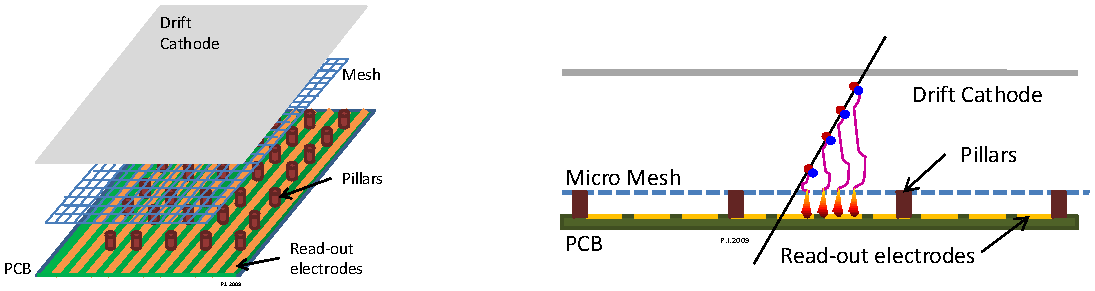
\includegraphics[width = 0.9\textwidth]{figures/micromegas.png}
%    \caption{Sketch the micromega operating principle. Positive high voltage is applied to the readout electrodes, which creates a strong field between the mesh and the readout electrodes, and a weaker field between the mesh and the drift cathode. Amplification takes place between the readout electrodes and the mesh. Figure from~\cite{nsw_tdr}}
%    \label{fig:micromega}
% \end{figure}

% --------------------------------------------------
\section{Small-strip thin gap chambers}
% --------------------------------------------------

\begin{figure}
    \centering
    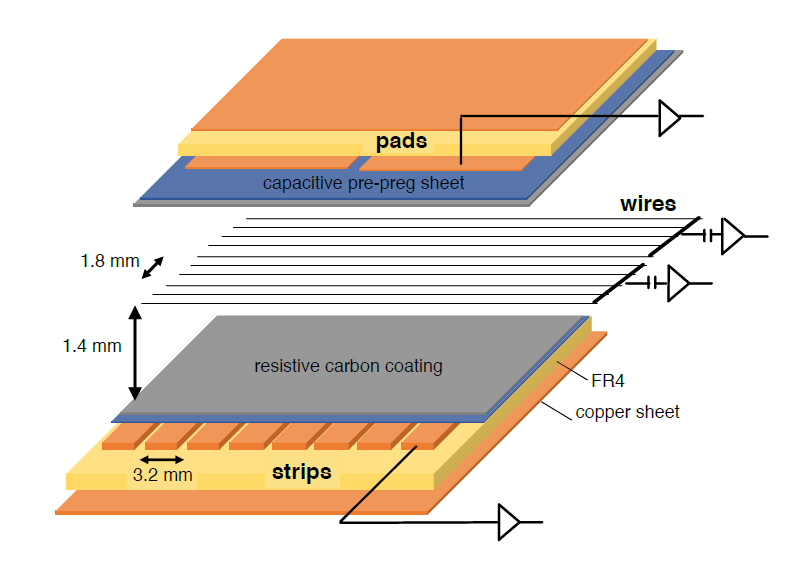
\includegraphics[width = 0.9\textwidth]{figures/stgc_internals.png}
    \caption{Interal structure of an sTGC, zoomed into the area under approximately 1 pad. High voltage is applied to wires suspended in the gas volume to create an electric field. A passing muon causes an ionization avalache that is picked up by the wire, strip and pad electrodes~\cite{lefebvre_precision_2020}.}
    \label{fig:stgc_internals}
\end{figure}

sTGCs are gas ionization chambers operated with a CO$_2$:n-pentane ratio of 55:45. Gold-plated tungsten wires, \SI{50}{\micro\meter} in diameter and with \SI{1.8}{mm} pitch, are suspended between two cathode planes made of FR-4, each \SI{1.4}{mm} away (see figure~\ref{fig:stgc_internals}. One cathode board is segmented into pads of varying area (around \SI{300}{cm^2} each), and the other segmented into strips of \SI{3.2}{mm} pitch, perpendicular to the wires. High voltage is applied to the wires and the cathode planes are grounded~\cite{nsw_tdr, perez-codina_small-strip_2016}. When a muon passes through, the gas is ionized and the electric field in the gas gap causes an ionization avalanche~\cite{townsend_electricity_1915}. The motion of the ions and electrons are picked up on the nearby wire, strip and pad electrodes. The resitivity of the carbon coating and capacitance of the pre-preg sheet tune the spread of the charge distribution~\cite{gatti_optimum_1979} and the speed of the response~\cite{battistoni_resistive_1982} to optimize the rate capability. The hatching of the strips and wires establishes a coordinate system from which to extract the coordinate of the muon as it passes through the layer~\cite{nsw_tdr}. 

% comment on "quick enough to be provided as input to the L1 trigger. Pg. 131 of NSW TDR states req' is under 1025 ns for phase-1, phase-2 will allow longer latency. Latency predictions are shown on pg. 146, but are mostly estimates. Not sure where these latencies are actually measured, nor what the phase-2 requirement is.
A 3-out-of-4 coincidence in the pad electrodes of a quadruplet will define a region of interest where the strip and wire electrodes should be readout. Then, a track segment with the required angular resolution can be constructed quickly enough to be provided as input to the hardware trigger~\cite{nsw_tdr}. The pad-triggering scheme greatly reduces the number of electrodes that require readout to provide the design track angular resolution of \SI{1}{mrad}. For the next run of ATLAS (run-3), the L1 trigger will pass if the track segment from the small wheel matches a region of interest defined by the TGCs of the big wheel~\cite{tdaq_phase1_tdr, nsw_tdr}. The increased angular resolution and $\eta$ coverage of the quadruplets will be an improvement in the triggering scheme over the current small wheel TGCs~\cite{nsw_tdr}. After the phase-II upgrade of the trigger and data acquisition system scheduled for $\sim$2025, which includes upgrades to the big wheel's angular resolution, there will only be a trigger if the combined track points back to the interaction point, increasing the muon $p_T$ resolution~\cite{nsw_tdr, tdaq_phase2_tdr}. 

Signal is readout from groups of successive wires, so the position resolution in the direction perpendicular to the wires is \SI{10}{mm}. The resolution in this direction is sufficient since it will give the symmetric azimuthal coordinate in ATLAS. Good resolution on the $\eta$ coordinate, perpendicular to the strips, is important~\cite{nsw_tdr}. The average single chamber position resolution in the strip coordinate was \SI{45}{\micro\meter} for perpendicular muon tracks as measured in a test beam~\cite{abusleme_performance_2016}~--- well within design specifications. When four sTGCs are glued together into a quadruplet the design angular resolution of \SI{1}{mrad} in the strip coordinate is achievable~\cite{nsw_tdr, perez-codina_small-strip_2016}. 

Therefore, sTGCs are able to meet the precision tracking and triggering goals they were designed for. To ensure they can deliver once installed in ATLAS, knowing the position of the strips to within their position resolution in the ATLAS coordinate system is necessary. The NSW alignment system, detailed in section~\ref{sec:nsw_alignment} monitors the position of alignment platforms installed on the surface of the wedges. The alignment platforms are installed with respect to an external reference on the sTGCs: two brass inserts on each strip layer on one of the angled sides of each quadruplet (shown in figure~\ref{fig:brasses}). So the challenge of positioning the strips in ATLAS was separated into two steps: first, position the strips with respect to the brass inserts; second use the alignment system to position the alignment platforms. The next section provides some pertinent details on the sTGC construction process, with steps that affect the position of the strips with respect to the brass inserts highlighted.
% The position of the strips can be separated into two stages. First, the NSW alignment system monitors the position of alignment platforms installed on the surface of the wedges, as detailed in section~\ref{nsw_alignment}. Second, the internal geometry of the chambers must be referenced with respect to the wedges. Parts of the sTGC construction process that affect the position of the strips are explained in section~\ref{sec:stgc_construction}. The chapter closes 

\begin{figure}
\centering
\begin{subfigure}{.5\textwidth}
  \centering
  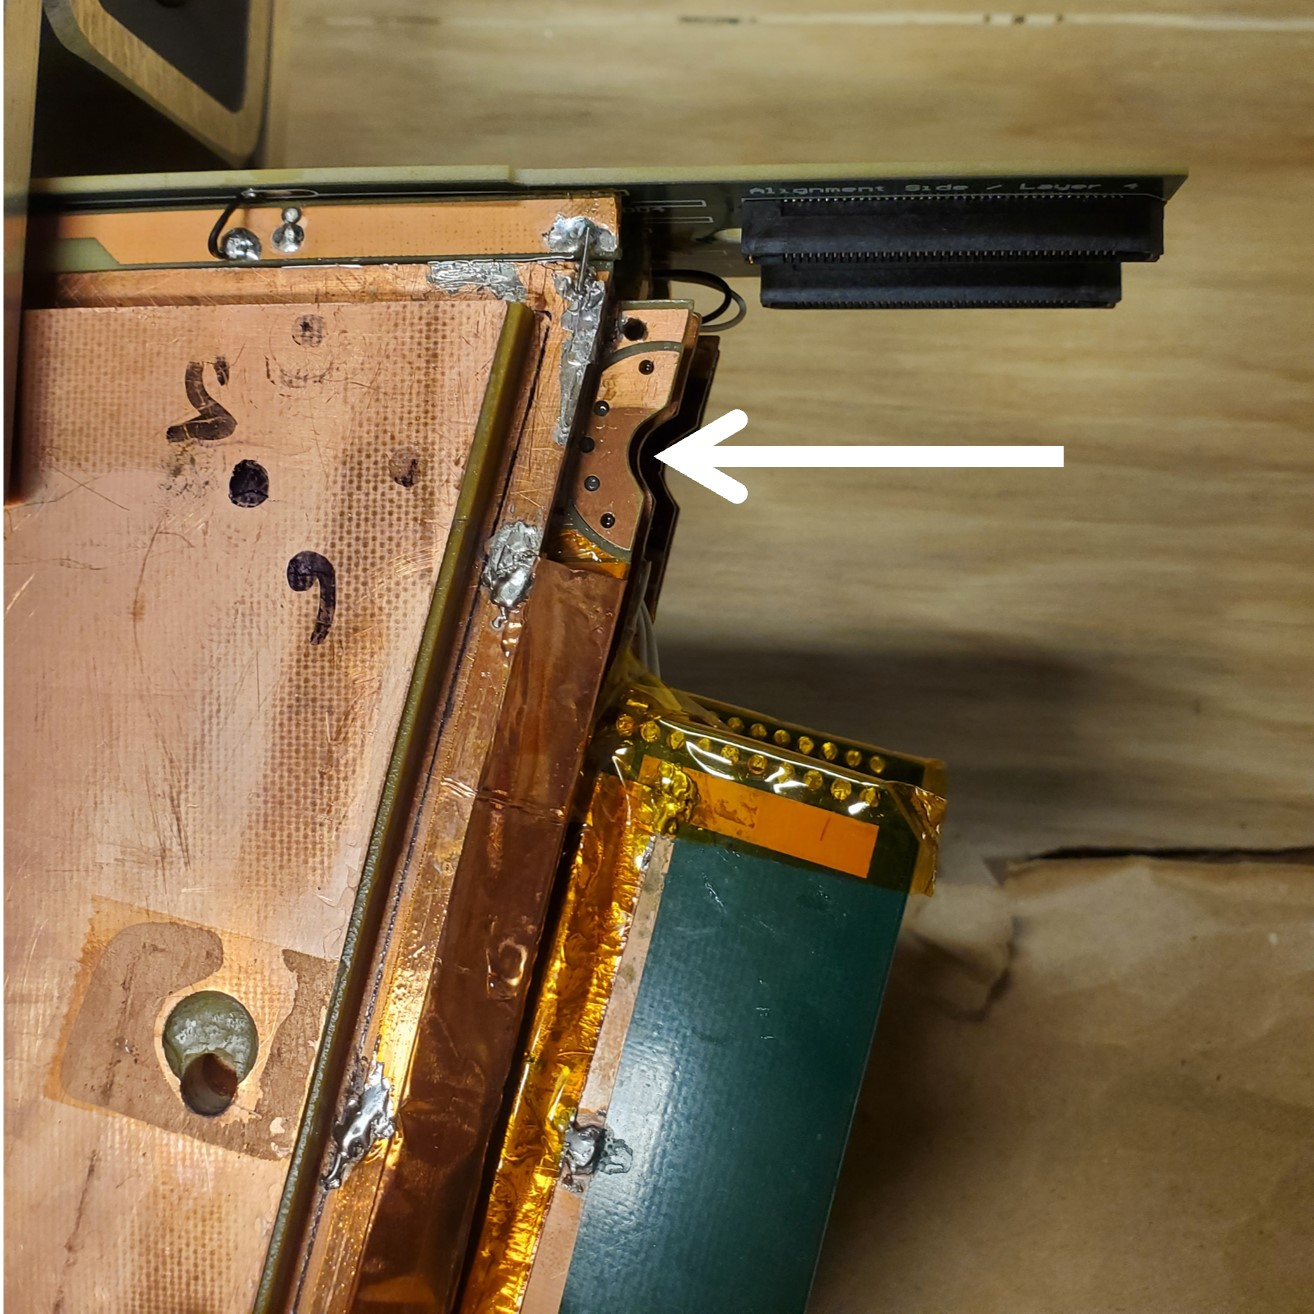
\includegraphics[width=\linewidth]{figures/brass_top.jpg}
  \caption{Brass insert near long edge.}
  \label{fig:brass_top}
\end{subfigure}%
\begin{subfigure}{.5\textwidth}
  \centering
  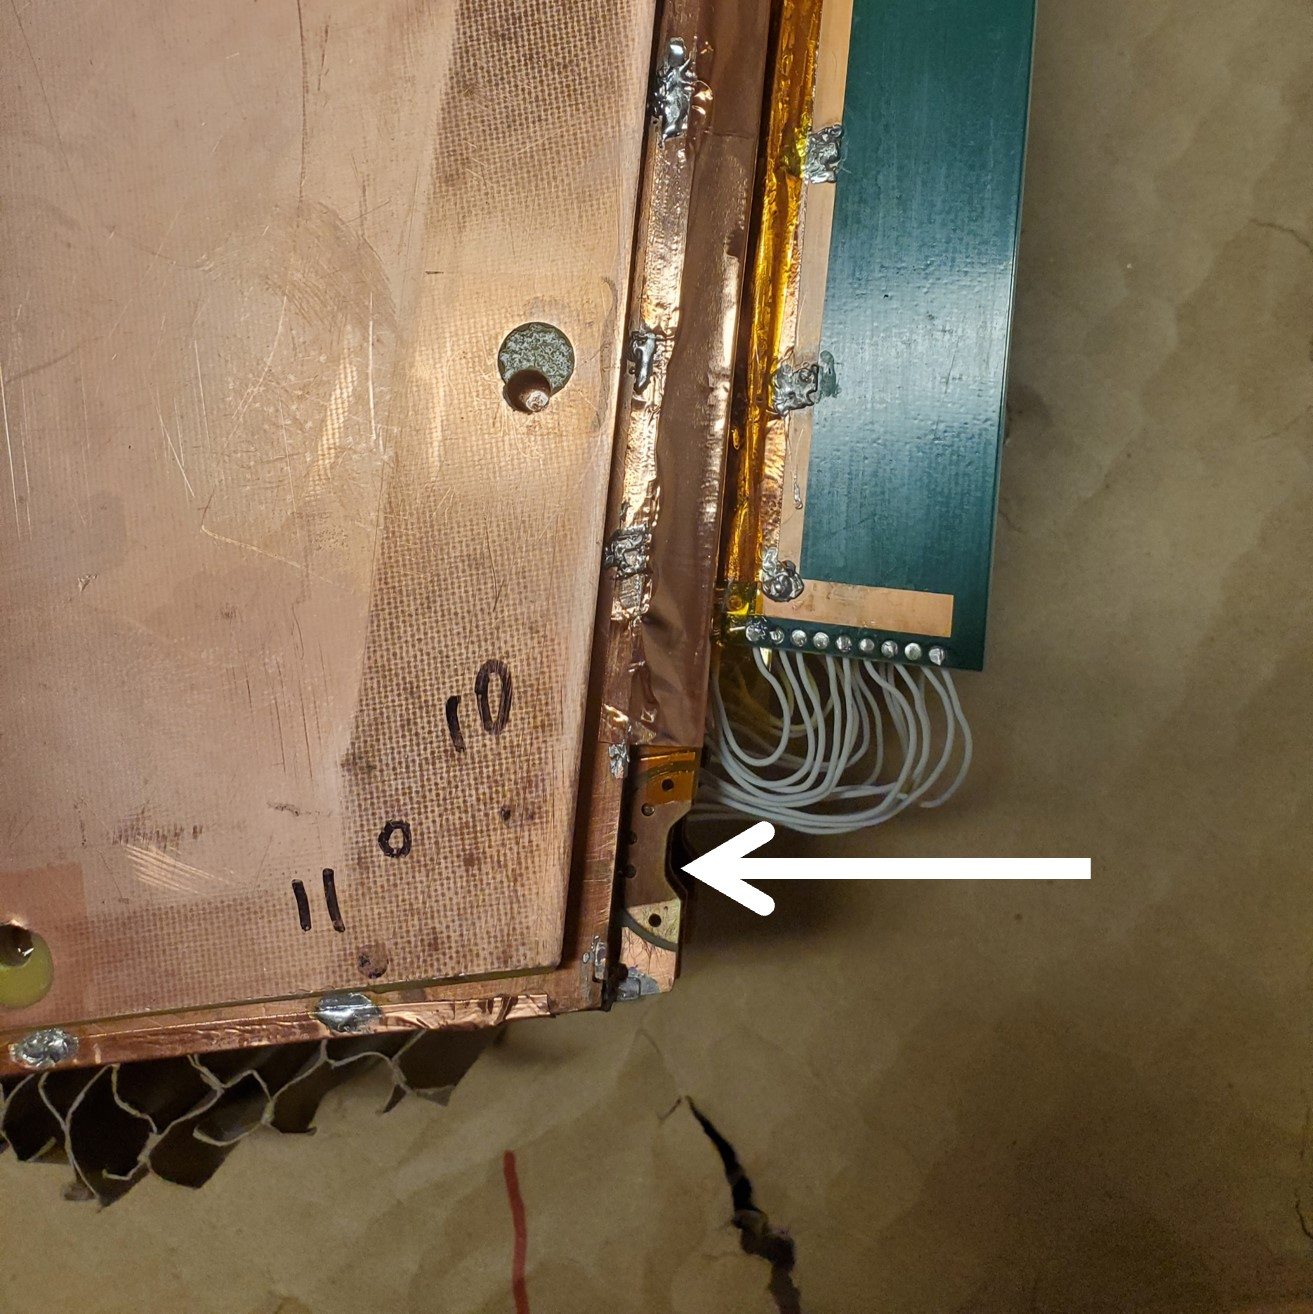
\includegraphics[width=\linewidth]{figures/brass_bottom.jpg}
  \caption{Brass insert near short edge.}
  \label{fig:brass_bottom}
\end{subfigure}
\caption{The brass inserts sticking out from the gas volumes of an sTGC quadruplet. These inserts were pressed against alignment pins when the individual sTGCs were being glued together.}
\label{fig:brasses}
\end{figure}

% However, the accuracy of the hit positions on each layer depends on how well the position of the strips are known in the ATLAS coordinate system. 

% Each strip cathode board has two brass inserts, one near the long edge and one near the short edge, pictured in figure~\ref{fig:brasses}. The inserts were used to align the strip layers of a quadruplet during construction. They were supposed to control the position of the strips to within \SI{40}{\micro\meter} within nominal. The idea was that the NSW alignment system would monitor the position of points on the surface of an sTGC wedge (discussed in section~\ref{sec:nsw_alignment}) and that the combined external and internal alignment uncertainty on the strip positions would be acceptably small for the precision tracking goals~\cite{nsw_tdr}. Uncontrolled offsets of strip positions on an sTGC layer will bias the reconstructed hit position and hence the track, reducing accuracy of the momentum measurement. To understand the source of offsets in strip positions and misalignments between strip layers, pertinent details of the sTGC construction process are presented in the next section.

% In addition, the sTGC quadruplets should be able to provide precision tracking within \SI{100}{\micro\meter} per plane in the event of a MM module failure.

% --------------------------------------------------
\section{sTGC Quadruplet Construction}
% --------------------------------------------------
\label{sec:stgc_construction}

Five countries were responsible for producing the sTGC modules of varying geometries for the NSW: Canada, Chile, China, Israel and Russia. Canada was responsible for 1/4 of the required sTGCs, of three different quadruplet geometries. The steps of the construction process in each country were similar~\cite{nsw_tdr}. The process followed in Canada is detailed.

TRIUMF in Vancouver, British Columbia was responsible for preparing the cathode boards. The boards were made and the electrodes etched on at a commercial laboratory, Triangle Labs, in Carson City, Nevada. Once completed they were sent to TRIUMF to be sprayed with graphite and otherwise prepared~\cite{carlson_results_2019}. The boards are commercial multilayer printed circuit boards, but the strip boards required precision machining to etch the strip pattern~\cite{nsw_tdr}. Triangle Labs also machined the two brass inserts into each strip board. A coordinate measuring machine (CMM) was used to digitize a set of reference strips. Four quality parameters describing non-conformities in the strip pattern of each board with respect to the brass inserts were derived from the data and the results are available on a QA/QC database. The parameters and the CMM data collection is described in full in Carlson's thesis~\cite{carlson_results_2019}.  Due to time constraints, tolerances on the non-conformities in the etched strip pattern with respect to the brass inserts were loosened, with the condition that the strip positions would have to be corrected for~\cite{carlson_results_2019}. 

The prepared boards were sent to Carleton University in Ottawa, Ontario for construction into sTGCs and quadruplets. First, the wires were wound around the pad cathode boards using a rotating table and the wires were soldered into place. A wound pad cathode board was held by vacuum on a granite table, flat to within \SI{20}{\micro\meter} and a strip cathode board glued on top to create an sTGC. Holding one sTGC flat with the vacuum, another was glued on top to create a doublet, then two doublets were glued together to create a quadruplet. When gluing sTGCs together, the brass inserts were pushed against alignment pins with the goal of keeping the strip layers aligned within tolerance. However, non-conformities in the shape of the brass inserts, non-conformities in the position of the alignment pins and shifts between strip layers while the glue cured resulted in misalignments between the brass inserts~-- and the strips~-- on successive layers. Precise alignment of the pad boards or wires with respect to the strip boards did not have to be so tightly controlled because pads do not measure the precision coordinate. 

The Carleton team finished the quadruplets by installing adaptor boards on the angled sides of each layer that allow front end electronics to be attached. Completed quadruplets were sent to McGill University where they were characterized with cosmic rays. The details of cosmic ray testing are described in chapter~\ref{chap:cosmics}. Quadruplets were then sent to CERN where they were assembled into wedges and alignment platforms installed. The alignment platforms were installed using a jig positioned with respect to the brass inserts. Completed wedges were assembled into sectors then installed on the NSWs.

% So, during cathode board construction the etched strip pattern could be shifted off of nominal with respect to the brass inserts. While gluing sTGCs together, non-conformities in the shapes of the brasses and the position of the alignment pins resulted in misalignments between the brass inserts that mean they are not a uniform reference for every layer of the quadruplet. 

The quadruplet construction process had two steps where strip positions could be shifted off of nominal. At board-level, there could be non-conformities in the etched strip pattern with respect to the brass inserts, described by the four quality parameters~\cite{carlson_results_2019}. At the quadruplet level, misalignments between the brass inserts and strips on different layers were introduced during the gluing. The result was that the brass inserts were not a reliable reference point and that the strips can be offset from their design position by up to hundreds of micrometers. Offsets in strip positions from nominal in Canadian quadruplets were shown to be random~\cite{carlson_results_2019}, so no one correction would suffice. The offsets must be measured and corrected for in the ATLAS offline software, \package{Athena}, which does the precision tracking. Understanding the work ongoing to make measurements of offsets and correct for them requires understanding the strategy of the NSW alignment system.

% Two sources of misalignment resulted at board level: non-conformities in the placement and shape of the brass inserts and non-conformities in the strip pattern. Carlson addressed the non-conformities in the strip pattern of Canadian cathode boards in his thesis~\cite{carlson_results_2019}. A coordinate measuring machine (CMM) or FaroArm was used to digitize the etched strip pattern of each board. Four quality parameters describing non-conformities in the strip pattern were derived from the data and the results are available on a QA/QC database. The parameters were offset, angle (rotation), scale and non-parallelism, defined in ful in Carlson' thesis. Often, alignment models only consider an offset and rotation. 

% Once the cathode boards were prepared, they were sent to TRIUMF in Vancouver, British Columbia to be sprayed with the graphite coating. After spraying, the coating was polished until the resistivity was between 90 and \SI{110}{\kilo\ohm}$/\msquare$, then wire support structures and frames were installed~\cite{nsw_tdr}. The completed boards were sent to Carleton university for construction into gas gaps and multiplets.

% First, anode wires were wound onto the the pad cathode boards using a rotating vacuum table. Then, a pad and strip cathode board has to be glued together to create an sTGC, two sTGCs glued together to create a doublet, and two doublets glued together to create a quadruplet. Gluing was done by holding one side of a cathode board in place with vacuum on a granite table, flat to within \SI{20}{\micro\meter}. A honey comb spacer separates each sTGC layer of a quadruplet. When closing a gas gap, micrometer misalignments between the strip and pad cathode boards do not matter since the pads do not measure precision coordinates. When gluing sTGCs into doublets however, alignment between strip layers had to be controlled by pushing the two brass inserts against alignment pins~--- similarly for gluing together doublets. Once a quadruplet was assembled, adapator boards used to route the electrodes' signals to the front end electronics were soldered on to the angled sides of the quadruplet~\cite{nsw_tdr}. 

% If you want to include the x-ray survery of the brass positions and the microscope method
% At every stage in the process quality control checks were in place for gas, high voltage, and alignment. For alignment, \textcolor{red}{the position of the brasses were recorded in 3D using an x-ray gun~\cite{nsw_tdr} \textit{--> Did this actually happen?}}~\cite{nsw_tdr} and alignment between strips visible outside a quadruplet was checked with a microscope~\cite{carlson_results_2019}. 

% Quality control tests of alignment, ability to hold high voltage, gas sealing etc. were undertaken at every stage in the construction process~-- details can be found in~\cite{nsw_tdr}. The final set of quality control checks and characterization was done at McGill University in Montreal, Quebec. Completed quadruplets were tested for gas leaks, noise and characterized with cosmic rays. The details of cosmic ray testing are described in chapter~\ref{chap:cosmics}.

% Once the quadruplets have been tested with cosmics rays, they are sent to CERN to be further tested, assembled into wedges then sectors, then installed on the NSWs. At the time of writing, all sectors have been installed on both wheels. The first NSW has been lowered into the ATLAS cavern and is being commissioned. The second is scheduled for installation in October, 2021.

% --------------------------------------------------
\section{NSW alignment}
% --------------------------------------------------
\label{sec:nsw_alignment}
%TODO : Mention Athena
% The idea of the NSW alignment system is presented in~\cite{nsw_tdr}, but the details have only been presented internally so far. The original goal of the alignment system was to provide the position with respect to one another of any three chambers traversable by a muon track with an accuracy of \SI{40}{\micro\meter} in the precision coordinate~\cite{nsw_tdr}. Likely for sTGCs, this will mean inputing the strip postions, or parameters to calculate the strip positions, into the ATLAS experiment's offline software, \package{Athena}.

%TODO : 
\textcolor{red}{What figures can I use to show the bars, the alignment jig, the platforms and the optical fibres?}.

The idea of the NSW alignment system is presented in~\cite{nsw_tdr}, but the details have only been presented internally so far. After the wedges are constructed, alignment platforms are installed on every sTGC quadruplet and optical fibres routed to them, as shown in figure~\ref{fig:alignment_platforms}. Light from the optical fibres will be monitored in real time by cameras (BCAMs) mounted on the alignment bars of the NSWs. The system will thus record the positions of the alignment platforms in the ATLAS coordinate system, accessible at any point during operation. % The final link in the sTGC alignment system requires knowing the position of the strips inside a chamber with respect to the alignment platforms.

\begin{figure}
    \centering
    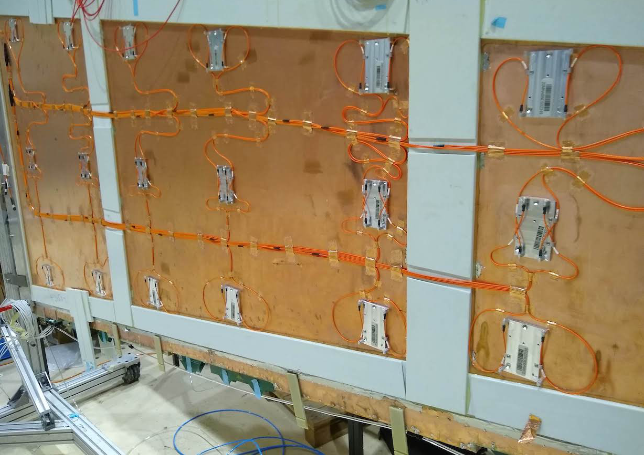
\includegraphics[width = 0.9\textwidth]{figures/alignment_platforms_lefebvre.png}
    \caption{An sTGC wedge with alignment platforms (silver) installed on the quadruplet. Optical fibres (orange) are routed to the alignment platforms. Cameras on the frame of the NSW will record light from the optical fibres to position the alignment platforms in the ATLAS coordinate system.}
    \label{fig:alignment_platforms}
\end{figure}

% If you want to mention the alignment jig in the last paragraph:
% They are positioned with the help of an alignment jig, which is like a frame that can be positioned on top of a wedge with cut outs indicating the correct position for the alignment platforms. The jig is positioned with respect to the brass inserts \textcolor{red}{[Benoit 2020-01-20, 2020-04-16 presentations]}.

% The goal was to control the position of the strips in the chamber to within ~\SI{40}{\micro\meter} for precision tracking goals~\cite{nsw_tdr} --- then knowing the position of the brass inserts with respect to the alignment platforms would allow the strips to be positioned accurately enough. That is the alignment scheme shown in solid arrows in figure~\ref{fig:alignment_elements}. Due to time constraints, tolerances on the non-conformities in the etched strip pattern were loosened, with the condition that the strips positions would have to be corrected for in the software~\cite{carlson_results_2019}. Then, non-conformities in the brass inserts, misalignment of the pins the brass inserts were pushed against, and shifts of the strip layers while the glue was curing resulted in misalignments between the brass inserts~-- and between the strips layers ~-- that prevent using the brasses as an external reference of the position of the strips. The misalignments between Canadian sTGCs were shown to be random~\cite{carlson_results_2019}, so no one correction would suffice.

% The original alignment scheme was to use the brass inserts as a reference between the alignment platforms and the individual strips, as shown in the solid arrows in figure~\ref{fig:alignment_elements}. \textcolor{red}{Due to time constraints, tolerances on the non-conformities in the etched strip pattern with respect to the brass inserts were loosened, with the condition that the strips positions would have to be corrected for. Corrections will happen in ATLAS offline software, \package{Athena}, that will do the precision tracking~\cite{carlson_results_2019}. --> MOVE THIS} Moreover, non-conformities in the shape of the brass inserts and the alignment pins added misalignment between the inserts of different layers~-- and between the strips of different layers~-- that prevent using the brass inserts as a reference. Offsets in strip positions from nominal in Canadian quadruplets were shown to be random~\cite{carlson_results_2019}, so no one correction would suffice.
%TODO : Did other construction sites have this problem?

\begin{figure}
    \centering
    
\includegraphics[width = 0.9\textwidth]{figures/alignment_system_element_relations.png}
    \caption{How the different elements of the sTGC alignment system relate to one another. The solid arrows denote the planned alignment scheme. The dashed arrow shows the modification being finalized now. This figure was originally designed by Dr. Benoit Lefebvre.}
    \label{fig:alignment_elements}
\end{figure}

The original alignment scheme was to use the brass inserts as a reference between the alignment platforms and the individual strips, as shown in the solid arrows in figure~\ref{fig:alignment_elements}~-- this will no longer work. The position of the alignment platforms will be known thanks to the alignment system, so a different method to get the position of the individual strips with respect to the alignment platform is currently in its final stages. It uses the yet-unmentioned x-ray dataset to calculate offsets of the strip pattern of an sTGC layer in a local area (local offset) with respect to the nominal geometry by analyzing the beam profile left by an x-ray gun attached to different positions on the alignment platforms. The alignment platforms provide the link to the nominal geometry because their position with respect to the strips is known in the case that the strips are perfectly etched and aligned. Effectively, the reference to the brass inserts is skipped, represented as the dashed line in figure~\ref{fig:alignment_elements}. 

The x-ray method does not have the sensitivity to measure the offset of each strip from nominal, but instead in a local area around the position of the gun. Local offsets are thus used to build an alignment model for each strip layer. Formally defined, an alignment model is a set of parameters used to estimate the true position of a strip given its nominal position. The alignment model currently being worked on takes x-ray and CMM data as input to calculate a global offsets and rotations of each strip layer with respect to nominal~\cite{lefebvre_precision_2020}. Without the x-ray dataset, there would be no input to the alignment model that takes into account inter-layer misalignments introduced in construction. 

Given that the x-ray local offsets can only be measured at positions where the gun can be attached and that they are an important part of the alignment scheme, the x-ray method needs to be validated. The goal of this thesis is to validate the x-ray local offsets while exploring how cosmics data complements and adds to the understanding of strip positions and overall alignment.

% --------------------------------------------------
% \section{Thesis motivation}
% --------------------------------------------------
%\textcolor{red}{It feels right to remind people of the goal of this work here, even though this is done in the introduction. Options: keep this section, remove this section; move the first two sentences of this section to the end of the NSW alignment section above for a briefer reminder. Thoughts?}

% Given that the x-ray local offsets can only be measured at positions where the gun can be attached and that they are an important part of the alignment scheme, the x-ray method needs to be validated. The goal of this thesis is to validate the x-ray local offsets while exploring how cosmics data complements and adds to the understanding of strip positions and overall alignment. Chapter~\ref{chap:lhc_atlas} presented the physics motivation of the HL-LHC and chapter~\ref{chap:nsw} motivated the NSW upgrade and the importance of alignment. Chapter~\ref{chap:cosmics} explains how cosmic muon data is collected, how it is used to calculate relative local offsets, and what information it gives about alignment. Chapter~\ref{chap:xray} explains how x-ray data is collected, how it is used to calculate local offsets, and how relative local offsets can be calculated for comparison to cosmics. Chapter~\ref{chap:comparison} compares the results of the two methods; and chapter~\ref{chap:outlook} contextualizes the results in terms of the alignment model and alignment system.

% Snippets
%The main dataset was collected using x-rays as the probe. The x-ray data has been combined with the CMM data to create an alignment model that can be used to estimate the position of each strip. The goal of this work was to validate the measurements of strip pattern offsets done with the x-ray dataset with the cosmic muon data. Currently, only modules made in Canada have been analyzed in this way, but the method applies for other countries that were able to collect cosmic muon data on multiple quadruplet layers. 

%Moreover, as-built alignment parameters must be measured and extracted to ensure proper function and provide a way to correct for misalignment. The next section breaks down the sTGC construction process to highlight the stages of alignment.
%All countries successfully finished delivering their modules this year, and the sectors have been installed on the NSWs. 






























